\documentclass[10pt]{beamer}

\usetheme[progressbar=frametitle]{metropolis}
\usepackage{appendixnumberbeamer}

\usepackage{booktabs}
\usepackage[scale=2]{ccicons}


\usepackage{pgfplots}
\usepgfplotslibrary{dateplot}

\usepackage{xspace}
\newcommand{\themename}{\textbf{\textsc{metropolis}}\xspace}

\title{Pub Quiz}
\subtitle{Nederlands}
\date{15/07/2019}
\date{}
\author{Slides available at \url{https://sinhp.github.io/blog/}}
\institute{Dizzy}
% \titlegraphic{\hfill\includegraphics[height=1.5cm]{logo.pdf}}
\usepackage{macro}
\usepackage[utf8]{inputenc}
\usepackage[T1]{fontenc}
\usepackage{parskip}
\usepackage{graphicx}
\usepackage{media9}

\setbeamertemplate{button}{\tikz
  \node[
  inner xsep=5pt,
  draw=structure!80,
  fill = white, 
  fill=structure!50,
  rounded corners=5pt]  {\color{white}\Large\insertbuttontext};}

\newcounter{vnum} %% vraag nummer
\newcounter{preframevnum}
\usecounter{vnum}
\newcommand{\vnummer}{\noindent\text{Vraag \arabic{vnum}}\refstepcounter{vnum}}
\setcounter{vnum}{1}

\pagenumbering{gobble}

\begin{document}

\maketitle

% \begin{frame}{Table of contents}
%   \setbeamertemplate{section in toc}[sections numbered]
%   \tableofcontents[hideallsubsections]
% \end{frame}

\section{Vragen}

\setcounter{preframevnum}{\value{vnum}}
\begin{frame}[fragile]{\vnummer \small  \hfill (\textsc{10 punten})}
\setcounter{vnum}{\value{preframevnum}}
\pause
\metroset{block=fill}
 \begin{alertblock}{Vraag}
 Noem het nummer en de zanger van het nummer dat het volgende bevat
in de tekst.  \hfill \\
 \pause
 \vspace{10pt}
\texttt{``Want je kunt niets zeker weten en alles gaat voorbij. Maar \ldots''} 
 \end{alertblock}
\pause
\vspace{5pt}
 \begin{exampleblock}{Wenk}
 \vspace{5pt}
 \begin{figure}
     \centering
     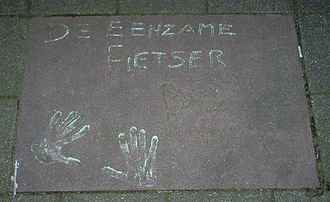
\includegraphics[scale=1.8]{WOF_Boudewijn_de_Groot.jpg}
     \caption{\textit{zijn/haar handafdrukken in de Walk of Fame te Rotterdam}}
     \label{fig:my_label}
 \end{figure}
 \end{exampleblock}
\end{frame}

\setcounter{preframevnum}{\value{vnum}}
\begin{frame}[fragile]{\vnummer \small \hfill (\textsc{8 punten})}
\setcounter{vnum}{\value{preframevnum}}
\pause
\metroset{block=fill}
 \begin{alertblock}{Vraag}
   Deze persoon 
   \begin{itemize}
       \item was volgens de Volkskrant Top 200 de invloedrijkste Nederlander van 2007, 2008, en 2009.
       \item is lid van D66.
       \item was eerder rector magnificus van de Erasmus Universiteit. 
       \item is lid van de raad van bestuur van ING.
   \end{itemize}
 \end{alertblock}
\end{frame}


\setcounter{preframevnum}{\value{vnum}}
\begin{frame}[fragile]{\vnummer \small \hfill (\textsc{12 punten})}
\setcounter{vnum}{\value{preframevnum}}
\pause
\metroset{block=fill}
 \begin{alertblock}{Vraag}
   Hoe oud is Arjen Lubach?
 \end{alertblock}
\end{frame}


\setcounter{preframevnum}{\value{vnum}}
\begin{frame}[fragile]{\vnummer \small \hfill (\textsc{16 punten})}
\setcounter{vnum}{\value{preframevnum}}
\pause
\href{https://youtu.be/slSXVoq75Yg?t=1423}{\beamergotobutton{Finale van WK '74}}
\pause
\metroset{block=fill}
 \begin{alertblock}{Vraag}
   welke van deze spelers in de finale van het Wereldkampioenschap voetbal 1974 in West-Duitsland niet tegen Duitsland speelde?  
   \begin{enumerate}
       \item \textsc{Johan Cruijff}
       \item \textsc{Ruud Krol}
       \item \textsc{Piet Schrijvers} 
       \item \textsc{René van de Kerkhof}
       \item \textsc{Arie Haan}
   \end{enumerate}
 \end{alertblock}
%  \begin{figure}[ht!]
%  % using a YouTube video
% \includemedia[
%   width=0.6\linewidth,height=0.3375\linewidth,
%   activate=pageopen,
%   flashvars={
%   modestbranding=1 % no YT logo in control bar
%   &autohide=1 % controlbar autohide
%   &showinfo=0 % no title and other info before start
%   &rel=0 % no related videos after end
% }
% ]{\includegraphics[width=0.6\linewidth]{048}}{https://www.youtube.com/watch?v=slSXVoq75Yg}
% \end{figure}
\end{frame}


\setcounter{preframevnum}{\value{vnum}}
\begin{frame}[fragile]{\vnummer \small \hfill (\textsc{10 punten})}
\setcounter{vnum}{\value{preframevnum}}
\pause
\metroset{block=fill}
 \begin{alertblock}{Vraag}
   Hoe zeg je ``Nederlands'' in het Russich?
 \end{alertblock}
\end{frame}


\setcounter{preframevnum}{\value{vnum}}
\begin{frame}[fragile]{\vnummer \small \hfill (\textsc{11 punten})}
\setcounter{vnum}{\value{preframevnum}}
\pause
\metroset{block=fill}
 \begin{alertblock}{Vraag}
   Hoe zeg je ``Hoe gaat het met jou?'' in het Fries?
 \end{alertblock}
\end{frame}



\setcounter{preframevnum}{\value{vnum}}
\begin{frame}[fragile]{\vnummer \small \hfill (\textsc{13 punten})}
\setcounter{vnum}{\value{preframevnum}}
\pause
\metroset{block=fill}
 \begin{alertblock}{Vraag}
   Van welke \texttt{Latijnse naam} was de naam \alert{Utrecht} later afgeleid?
 \end{alertblock}
\end{frame}


\setcounter{preframevnum}{\value{vnum}}
\begin{frame}[fragile]{\vnummer \small \hfill (\textsc{10 punten})}
\setcounter{vnum}{\value{preframevnum}}
\pause
\textbf{\texttt{Het Spreekwoorden spel: raad het spreekwoord!}}\\
\vspace{20pt}
\texttt{Bijvoorbeelden:}
  \begin{columns}[T,onlytextwidth]
    \column{0.5\textwidth}
      \begin{itemize}
        \item Milk 
      \end{itemize}

    \column{0.5\textwidth}
      \begin{itemize}
          \item First,
      \end{itemize}

  \end{columns}




\metroset{block=fill}
 \begin{alertblock}{Vraag}
   
 \end{alertblock}
\end{frame}



%%%%%%%%
%%%%%%%%
\section{Einde van vraagen}



%%% -------------
%%% -------------
\section{Aantowoorden}
\setcounter{vnum}{1}

\setcounter{preframevnum}{\value{vnum}}
\begin{frame}[fragile]{\vnummer \small \hfill (\textsc{10 punten})}
\setcounter{vnum}{\value{preframevnum}}
\textbf{\texttt{Avond van Boudewijn de Groot}}\\
\vspace{10pt}
\small{\textit{ Nu hoef je nooit je jas meer aan te trekken\\
en te hopen dat je licht het doet.\\
Laat buiten de stormwind nu maar razen in het donker\\
want binnen is het warm en licht en goed.\\
Hand in hand naar buiten kijken waar de regen valt.\\
Ik zie het vuur van hoop en twijfel in je ogen\\
en ik ken je diepste angst.\\
\textbf{\alert{Want je kunt niets zeker weten en alles gaat voorbij.}}\\
Maar ik geloof, ik geloof, ik geloof,\\
ik geloof, ik geloof in jou en mij.\\
En als je 's morgens opstaat ben ik bij je\\
en misschien heb ik al thee gezet.\\
En als de zon schijnt buiten gaan we lopen door de duinen\\
en als het regent gaan we terug in bed.\\
Uren langzaam wakker worden, zwevend door de tijd,\\
ik zie het licht door de gordijnen en ik weet:\\
het verleden geeft geen zekerheid \ldots \\}}
\end{frame}

\setcounter{preframevnum}{\value{vnum}}
\begin{frame}[fragile]{\vnummer \small \hfill (\textsc{8 punten})}
\setcounter{vnum}{\value{preframevnum}}
\textbf{\texttt{Alexander Rinnooy Kan}}\\
\vspace{10pt}
\url{https://www.volkskrant.nl/nieuws-achtergrond/rinnooy-kan-invloedrijkste-nederlander~b61a091d/}
\end{frame}


\setcounter{preframevnum}{\value{vnum}}
\begin{frame}[fragile]{\vnummer \small \hfill (\textsc{12 punten})}
\setcounter{vnum}{\value{preframevnum}}
Arjen Lubach werd geboren op 22 oktober 1979 in Groningen. \\ 
\vspace{10pt}
\begin{center}
  Daarom is hij  \alert{\textbf{\texttt{39 jaar oud}}}.  
\end{center}
\end{frame}

\setcounter{preframevnum}{\value{vnum}}
\begin{frame}[fragile]{\vnummer \small \hfill (\textsc{16 punten})}
\setcounter{vnum}{\value{preframevnum}}
Onder leiding van Rinus Michels werd de finale gehaald, waarin het Nederlandse team van West-Duitsland verloor met 2-1, ondanks een geweldige prestatie.\\
\vspace{5pt}
\pause 
\begin{figure}
\centering
    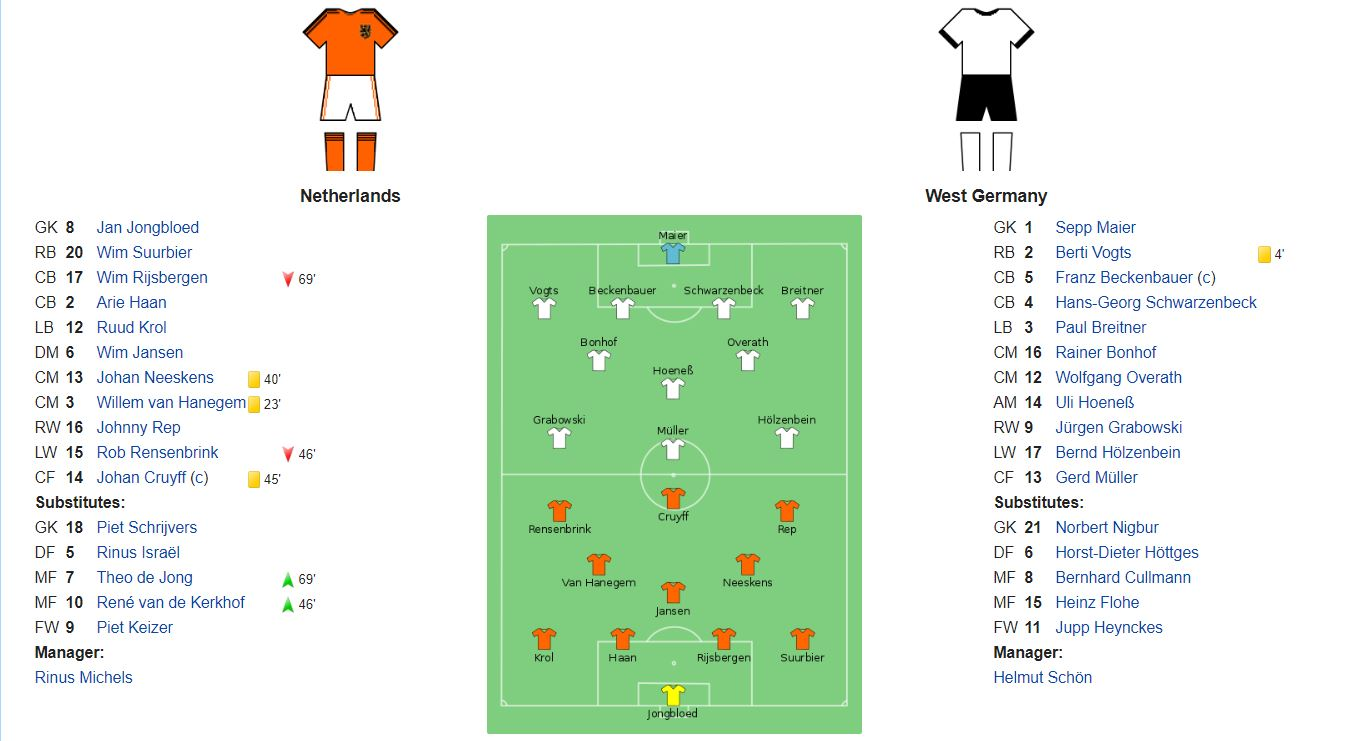
\includegraphics[scale=0.32]{Duitsland-vs-Nederland.JPG}
\end{figure}
\pause
De Aantwoord is \alert{Piet Schrijvers}. Hij was de reserve keeper. \\ 
\end{frame}


\setcounter{preframevnum}{\value{vnum}}
\begin{frame}[fragile]{\vnummer \small \hfill (\textsc{10 punten})}
\setcounter{vnum}{\value{preframevnum}}
\begin{center}
  \alert{\textbf{\texttt{Goll\,andskij}}}.  
\end{center}
\end{frame}


\setcounter{preframevnum}{\value{vnum}}
\begin{frame}[fragile]{\vnummer \small \hfill (\textsc{11 punten})}
\setcounter{vnum}{\value{preframevnum}}
\begin{center}
  \alert{\textbf{\texttt{Hoe giet it mei dy?}}}.  
\end{center}
\end{frame}


\setcounter{preframevnum}{\value{vnum}}
\begin{frame}[fragile]{\vnummer \small \hfill (\textsc{11 punten})}
\setcounter{vnum}{\value{preframevnum}}
\alert{\textbf{\texttt{Traiectum}}}
\pause
\vspace{10pt}
\ilum{Onder het huidige Domplein in {\color{utrechtYellow}{Utrecht}} zijn nog resten annwezig van een fort uit de Romeinse tijd. Dat fort, gelegen langs de rivier de Rijn, droeg de Latijnse naam \texttt{Traiectum}, wat `doorwaadbare plaats' (in een rivier) of `overgang' betekent. Van deze naam is later de naam Utrecht afgeleid. \textit{`Utrecht'} is een samenstelling van {\color{utrechtYellow}{\textit{uut}}} (Oudnederlands voor `uit') en {\color{utrechtYellow}{\textit{Trecht}}} (van Traiectum). }
\pause 
\ilum{In 1290, een dichter voegde `uut' toe aan `Trecht'.}

\end{frame}







%%%------------------------------------------------------------------------------------------------
\begin{frame}{Lists}
  \begin{columns}[T,onlytextwidth]
    \column{0.33\textwidth}
      Items
      \begin{itemize}
        \item Milk \item Eggs \item Potatos
      \end{itemize}

    \column{0.33\textwidth}
      Enumerations
      \begin{enumerate}
        \item First, \item Second and \item Last.
      \end{enumerate}

    \column{0.33\textwidth}
      Descriptions
      \begin{description}
        \item[PowerPoint] Meeh. \item[Beamer] Yeeeha.
      \end{description}
  \end{columns}
\end{frame}


\begin{frame}{Tables}
  \begin{table}
    \caption{Largest cities in the world (source: Wikipedia)}
    \begin{tabular}{lr}
      \toprule
      City & Population\\
      \midrule
      Mexico City & 20,116,842\\
      Shanghai & 19,210,000\\
      Peking & 15,796,450\\
      Istanbul & 14,160,467\\
      \bottomrule
    \end{tabular}
  \end{table}
\end{frame}
\begin{frame}{Blocks}
  Three different block environments are pre-defined and may be styled with an
  optional background color.

  \begin{columns}[T,onlytextwidth]
    \column{0.5\textwidth}
      \begin{block}{Default}
        Block content.
      \end{block}

      \begin{alertblock}{Alert}
        Block content.
      \end{alertblock}

      \begin{exampleblock}{Example}
        Block content.
      \end{exampleblock}

    \column{0.5\textwidth}

      \metroset{block=fill}

      \begin{block}{Default}
        Block content.
      \end{block}

      \begin{alertblock}{Alert}
        Block content.
      \end{alertblock}

      \begin{exampleblock}{Example}
        Block content.
      \end{exampleblock}

  \end{columns}
\end{frame}


% \begin{frame}{Line plots}
%   \begin{figure}
%     \begin{tikzpicture}
%       \begin{axis}[
%         mlineplot,
%         width=0.9\textwidth,
%         height=6cm,
%       ]

%         \addplot {sin(deg(x))};
%         \addplot+[samples=100] {sin(deg(2*x))};

%       \end{axis}
%     \end{tikzpicture}
%   \end{figure}
% \end{frame}
% \begin{frame}{Bar charts}
%   \begin{figure}
%     \begin{tikzpicture}
%       \begin{axis}[
%         mbarplot,
%         xlabel={Foo},
%         ylabel={Bar},
%         width=0.9\textwidth,
%         height=6cm,
%       ]

%       \addplot plot coordinates {(1, 20) (2, 25) (3, 22.4) (4, 12.4)};
%       \addplot plot coordinates {(1, 18) (2, 24) (3, 23.5) (4, 13.2)};
%       \addplot plot coordinates {(1, 10) (2, 19) (3, 25) (4, 15.2)};

%       \legend{lorem, ipsum, dolor}

%       \end{axis}
%     \end{tikzpicture}
%   \end{figure}
% \end{frame}



\section{Conclusion}

% \begin{frame}{Summary}

%   Get the source of this theme and the demo presentation from

%   \begin{center}\url{github.com/matze/mtheme}\end{center}

%   The theme \emph{itself} is licensed under a
%   \href{http://creativecommons.org/licenses/by-sa/4.0/}{Creative Commons
%   Attribution-ShareAlike 4.0 International License}.

%   \begin{center}\ccbysa\end{center}

% \end{frame}

{\setbeamercolor{palette primary}{fg=black, bg=yellow}
\begin{frame}[standout]
  Questions?
\end{frame}
}


\end{document}
